\documentclass[final]{beamer}

\usepackage[T1]{fontenc}
\usepackage{lmodern}
\usepackage{anyfontsize}

\usepackage[orientation=portrait,size=a0,scale=1.5]{beamerposter}
\usetheme{gemini}
\usecolortheme{nott}

\usepackage{amsmath}
\usepackage{amssymb}
\usepackage{graphicx}
\usepackage{booktabs}
\usepackage{microtype}
\usepackage{csquotes}
\usepackage[backend=biber,style=numeric]{biblatex}
\usepackage{tikz}
\usepackage{pgfplots}
\usepackage[dvipsnames]{xcolor}
\pgfplotsset{compat=1.18}

\usepackage{hyperref}
\usepackage{cleveref}

\addbibresource{../chiral-references.bib}

\setbeamersize{text margin left=3cm,text margin right=3cm}
\setbeamertemplate{navigation symbols}{}

\title{Ecuación de Dirac Quiral: \\
Grados de Libertad y Masa de los Neutrinos}
\author{Julian L. Avila-Martinez$^{1}$, Laura Y. Herrera-Martinez$^{1}$,
Sebastian Rodriguez-Garcia$^{1}$, J. Alfonso Leyva$^{2}$}
\institute{$^{1}$Física, Universidad Distrital Francisco José de Caldas \\
$^{2}$Pontificia Universidad Javeriana}
\newcommand{\email}{jlavilam@udistrital.edu.co}

% Upper Header Template
\setbeamertemplate{headline}{
  \begin{tikzpicture}[remember picture, overlay]
    \usebeamercolor{headline}
    \fill[bg] (current page.north west)
      rectangle ([yshift=-15.5cm]current page.north east);

    \node[anchor=north east, inner sep=0pt, align=center]
      at ([xshift=-2cm, yshift=-3cm]current page.north east) {
        {\fontsize{70pt}{85pt}\selectfont FP6-P3} \\[1cm]
        
\includegraphics[height=5cm]{./figures/qr-git.pdf}
      };

    % Left-aligned title block
    \node[anchor=north west, align=left, text=white, text width=0.9\paperwidth]
      at ([xshift=3cm, yshift=-2cm]current page.north west) {
        {\fontsize{70pt}{85pt}\selectfont \spaceskip=0.4em \textbf{\inserttitle} \par}
        \vspace{0.6cm}
        {\large \insertauthor \par}
        \vspace{0.25cm}
        {\normalsize \insertinstitute \par}
        \vspace{0.25cm}
        {\normalsize \texttt{\email} \par}
      };
  \end{tikzpicture}
  \vspace{12.5cm}
}

% Lower Footer Template
\setbeamertemplate{footline}{
  \begin{tikzpicture}[remember picture, overlay]
    \usebeamercolor{headline}
    \node[anchor=south] at ([yshift=3.5cm]current page.south) {
        \makebox[0.9\paperwidth][c]{
          
\includegraphics[height=10cm]{./figures/logo-ud-ver.pdf}\hfill
          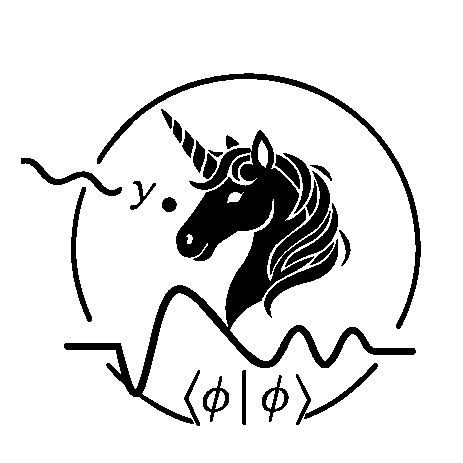
\includegraphics[height=10cm]{./figures/chap-logo.pdf}\hfill
          
\includegraphics[height=7cm]{./figures/acolfisica.pdf}\hfill
          
\includegraphics[height=8cm]{./figures/cifi-sema.pdf}
        }
      };
  \end{tikzpicture}
}

\begin{document}
\begin{frame}[t]

  \vspace{3cm}

  \begin{block}{Resumen}
  \begin{itemize}
    \item \textbf{Problema} La ecuación de Dirac quiral incorpora un ángulo
      en la dinámica del campo espinorial. \\
      El ángulo quiral induce un término de masa pseudoescalar. \\
      El lagrangiano de Yukawa se anula para las excitaciones levógiras,
      prediciendo neutrinos con masa nula.

    \item \textbf{Objetivo} Implementar un mecanismo seesaw quiral para generar
      dinámicamente un término de masa de Majorana.

    \item \textbf{Resultados} La estructura produce una excitación dextrógira
      estéril masiva y un campo activo levógiro con masa casi nula. \\
      El límite de ángulo quiral nulo recupera la teoría estándar.
  \end{itemize}
\end{block}


  \vspace{-1.5cm}

  \begin{columns}[t]
    \begin{column}{0.48\textwidth}
      \begin{block}{¿Qué es la Quiralidad?}
  Propiedad invariante de Lorentz que caracteriza la transformación de
  las componentes espinoriales bajo boosts $\Lambda$:
  \begin{gather}
    \psi = \psi_L + \psi_R, \\
    \psi_L \to \Lambda \psi_L \quad , \quad \psi_R \to \Lambda^{-1} \psi_R.
  \end{gather}

  Las componentes transforman según representaciones inequivalentes del
  grupo de Lorentz:
  \begin{itemize}
    \item Levógira ($\psi_L$): $(1/2, 0)$
    \item Dextrógira ($\psi_R$): $(0, 1/2)$
  \end{itemize}
\end{block}


      \begin{alertblock}{Ecuación de Dirac con Simetría Quiral}
  \begin{equation}\label{eq:decs}
    \left( i \gamma^\mu \partial_\mu - m e^{- i 2 \alpha \gamma^5} \right) \psi = 0
  \end{equation}

  La dinámica del campo espinorial queda determinada por las representaciones
  irreducibles del grupo de Poincaré bajo tres requerimientos axiomáticos
  fundamentales:
  \begin{itemize}
    \item \emph{Invariancia de Poincaré:} Equivalencia física estricta bajo
      transformaciones de Lorentz y traslaciones espaciotemporales.
    \item \emph{Invariancia Gauge:} Generación de interacciones físicas como
      consecuencia directa de la simetría local del lagrangiano.
    \item \emph{Localidad:} Restricción de la interacción causal a campos
      evaluados en el mismo punto del espaciotiempo.
  \end{itemize}
\end{alertblock}


      \begin{block}{El Lagrangiano Quiral de Yukawa}
  El acoplamiento de Yukawa con sectores escalares y pseudoescalares
  adopta la forma
  \begin{equation}
    \mathcal{L}_{Y} = -\frac{\lambda_{1}v_{1}}{\sqrt{2}}\overline{\psi}\psi
    - \frac{\lambda_{2}v_{2}}{\sqrt{2}}\overline{\psi}\gamma^{5}\psi.
  \end{equation}

  Mediante los parámetros de masa escalar $M$ y pseudoescalar $\tilde{M}$,
  la densidad lagrangiana se expresa en función de las proyecciones
  quirales como
  \begin{equation}
    \mathcal{L}_{\text{Dirac}} = \overline{\psi}_{L}(M+\tilde{M})\psi_{R}
    + \overline{\psi}_{R}(M-\tilde{M})\psi_{L}.
  \end{equation}
\end{block}

    \end{column}
    \begin{column}{0.48\textwidth}
      \begin{alertblock}{El Problema de la Masa Nula}
  Si se impone una restricción estricta asumiendo únicamente campos
  levógiros ($P_L \nu = \nu$), los bilineales escalares y pseudoescalares
  se anulan idénticamente
  \begin{gather}
    \overline{\nu} \nu = \overline{\nu} P_R P_L \nu = 0 \\
    \overline{\nu} \gamma^5 \nu = \overline{\nu} \gamma^5 P_R P_L \nu = 0
  \end{gather}

  El lagrangiano de Yukawa resulta trivial, prediciendo una masa nula para
  el neutrino activo.
\end{alertblock}


      \begin{block}{Mecanismo Seesaw Quiral}
  La supresión natural de la masa exige la inclusión de un término de Majorana
  para la componente dextrógira estéril. El lagrangiano extendido es
  \begin{equation}
    \mathcal{L}_{\text{Mass}} = \overline{\nu}_{L}M_{D}\nu_{R} 
    + \frac{1}{2}\overline{\nu_{R}^{c}}M_{R}\nu_{R} + h.c.
  \end{equation}

  Bajo la condición de una masa activa intrínseca nula ($M_L \approx 0$) y 
  definiendo la masa de Dirac quiral como $M_D = m e^{-i\alpha}$, la dinámica 
  queda determinada por la matriz de masa
  \begin{equation}
    \mathcal{M} = \begin{pmatrix} 
      0 & m e^{-i\alpha} \\ 
      m e^{-i\alpha} & M_R 
    \end{pmatrix}.
  \end{equation}

  En el régimen de alta energía ($M_R \gg m$), la diagonalización de la matriz 
  revela dos estados físicos con valores propios bien diferenciados:
  \begin{equation}
    m_1 \approx \frac{m^2}{M_R} e^{-2i\alpha}, \quad m_2 \approx M_R.
  \end{equation}

  Aquí, $m_1$ corresponde al neutrino activo levógiro, mientras que $m_2$ 
  representa la excitación dextrógira estéril. 
  El ángulo quiral $\alpha$ determina unívocamente la fase del neutrino activo, 
  constituyendo una fuente geométrica directa de violación CP leptónica.
\end{block}

      \vspace{-0.5cm}

      \begin{block}{Referencias}
        Referencias Completas escaneando el código QR.
        \footnotesize{\printbibliography}
        \nocite{watsonChiralSymmetryDirac2020}
        \nocite{Avila2025ChiralDirac}
      \end{block}

    \end{column}
  \end{columns}

\end{frame}
\end{document}
